% Preamble
\documentclass[17pt]{article}

% Math related packages.
\usepackage{amsfonts, amsthm, amsmath, amssymb, amstext}
\usepackage{mathtools}
\usepackage{physics}
\usepackage{cancel, textcomp}
\usepackage[mathscr]{euscript}
\usepackage[nointegrals]{wasysym}
\usepackage[left=3cm, right=3cm, top=1.5cm, bottom=1.5cm]{geometry}

\usepackage{esvect}
\usepackage{IEEEtrantools}

% Font related packages.
\usepackage[french]{babel}
\usepackage[unicode]{hyperref}
\usepackage[fontsize = 10pt]{scrextend}
\usepackage[T1]{fontenc}
\usepackage[utf8]{inputenc}
\usepackage[finemath]{kotex}
\usepackage{dhucs-nanumfont}
\usepackage{mathpazo}
\usepackage{FiraMono}
\usepackage{mathrsfs}

% Other
\usepackage{enumerate}
\usepackage[shortlabels]{enumitem}
\usepackage{tabularx}
\usepackage[object=vectorian]{pgfornament}
\usepackage{pgf}
\usepackage{pgfpages}
\usepackage[european,straightvoltages]{circuitikz}
\usepackage{scalerel}
\usepackage{stackengine}


% A more colorful world.
\usepackage{xcolor}

% Display Source Code
\usepackage{listings}
\lstset{
    language=C,
    basicstyle=\small\ttfamily\mdseries,
    numberstyle=\color{gray},
    stringstyle=\color[HTML]{933797},
    commentstyle=\color[HTML]{228B22},
    emph={[2]from,with,import,as,pass,return,and,or,not},
    emphstyle={[2]\color[HTML]{DD52F0}},
    emph={[3]range,format,enumerate,print},
    emphstyle={[3]\color[HTML]{D17032}},
    emph={[4]if,elif,else,for,while,in,def,lambda,int,float,all,len},
    emphstyle={[4]\color{blue}},
    emph={[5]abs},
    emphstyle={[5]\color{black}},
    showstringspaces=false,
    breaklines=true,
    prebreak=\mbox{{\color{gray}\tiny$\searrow$}},
    numbers=left
}

% OPTIONS
\everymath\expandafter{\the\everymath\displaystyle}

% Tikz libraries
\usetikzlibrary{angles, quotes}

% COMMANDS
\newcommand{\f}[1]{\texttt{#1}}
\newcommand{\sct}[1]{
	\begin{center}
		\Large\textbf{#1}
	\end{center}
}
\newcommand{\subsct}[1]{
	\begin{center}
		\large\textbf{#1}
	\end{center}
}
\newcommand{\inl}[2]{[\![#1, #2]\!]}
\newcommand{\q}[1]{\textbf{#1.}\quad}
\newcommand{\urlsymbol}{\kern1pt\vbox to .5ex{}\raise.10ex\hbox{\pdfliteral{%
    q .8 0 0 .8 0 0 cm
    2.5 5 m 1 j 1 J .8 w
    1 5 l 0 5 0 4 y 0 1 l 0 0 1 0 y 4 0 l 5 0 5 1 y 5 2.5 l S
    3 3 m 6 6 l S 4 6 m 6 6 l 6 4 l S
Q}}\kern5pt}

\newcounter{iloop}
\newcommand\openbigstar[1][0.7]{%
  \scalerel*{%
    \stackinset{c}{-.125pt}{c}{}{\scalebox{#1}{\color{white}{$\bigstar$}}}{%
      $\bigstar$}%
  }{\bigstar}
}
\newcommand{\Stars}[1]{\ensuremath{%
\pgfmathtruncatemacro{\imax}{ifthenelse(int(#1)==#1,#1-1,#1)}%
\pgfmathsetmacro{\xrest}{0.9*(1-#1+\imax)}%
\setcounter{iloop}{0}%
\loop\stepcounter{iloop}\ifnum\value{iloop}<\the\numexpr\imax+1
\bigstar\repeat
\openbigstar[\xrest]%
\setcounter{iloop}{0}%
\loop\stepcounter{iloop}\ifnum\value{iloop}<\the\numexpr5-\imax\relax
\openbigstar[.9]\repeat}}

\def\N{\mathbb N}
\def\Z{\mathbb Z}
\def\Q{\mathbb Q}
\def\R{\mathbb R}
\def\Rpe{\mathbb R_+^*}
\def\C{\mathbb C}
\def\K{\mathbb K}
\def\L{\mathbb L}

\def\P{\mathscr{P}}

\def\ssi{\Leftrightarrow}
\def\Ssi{\Longleftrightarrow}
\def\implique{\Longrightarrow}

\def\sep{\noindent\makebox[\linewidth]{\rule{\paperwidth}{0.4pt}}}

% CUSTOM TITLE
\makeatletter
\def\@maketitle{%
	\newpage
	%  \null% DELETED
	%  \vskip 2em% DELETED
	\begin{center}%
		\let \footnote \thanks
		{\LARGE \@title \par}%
		\vskip 1em%
		{\large
			\lineskip .5em%
			\begin{tabular}[t]{c}%
				\@author
			\end{tabular}\par}%
		\vskip 1em%
		{\large \@date}%
		\vskip 1cm%
	\end{center}%
	\par
	\vskip -1em}
\makeatother

\title{TP11 – Pendule non-linéaire}
\author{Amar AHMANE\\ MP2I}

\begin{document}
	\maketitle
	
	Le but de ce TP est de résoudre analytiquement une équation différentielle non-linéaire décrivant un système physique : il s'agira ici du pendule simple qui ne présente pas de solution analytique simple. 
	\subsection*{Étude théorique et équations utilisées}
	Le schéma ci-dessous représente le système physique étudié
	\begin{center}
		\begin{tikzpicture}
			\coordinate (origin) at (0, -0.2);
			\node (originbullet) at (origin) {$\bullet$};
			\node (O) at (originbullet) [above left] {$O$};
			\coordinate (masscord) at (1.4, -2.8);
			\coordinate (masscorda) at (1.2626, -2.8);
			\coordinate (gorigin) at (-1, -0.5);
			\node (mass) at (masscord) [below left=0.4em] {$M$};
			\coordinate (up) at (0, 0);
			\coordinate (down) at (0, -3.5);
		
			\draw[dashed] (up) -- (down);
			\draw[thick] (origin) -- (masscord) node [below, right=0.5em, midway] {$\ell$};
			\draw pic [draw, ->, angle radius=12mm, angle eccentricity=0.45mm, "$\theta$"] {angle = down--up--masscorda};
			\draw[dashed, color=gray!50] let \p1 = ($(masscord) - (origin)$), \n1 = {veclen(\x1,\y1)} in (origin) +(-45:\n1) arc [start angle = -45, delta angle = -90, radius = \n1];
			\draw[very thick, color=blue!60, -latex] (masscord) -- ++(0, -1.5) node [below] {$\overrightarrow{P}$};
			\draw[very thick, color=green!60!black!40, -latex] let \p1 = (origin), 
														 \p2 = ($(masscord) - (origin)$),
														 \n1 = {-acos(\y2/veclen(\x2, \y2))}
												in (masscord) -- +(\n1+90:-1.5) node [left=0.3em, below=0.25em] {$\overrightarrow{T}$};
			\draw[very thick, color=black!40, -latex] let \p1 = (origin), 
														 \p2 = ($(masscord) - (origin)$),
														 \n1 = {-acos(\y2/veclen(\x2, \y2))}
												in (masscord) -- +(\n1:-1) node [above=0.4em, left=0.4em] {$\overrightarrow{e_\theta}$};
			\draw[very thick, color=black!40, -latex] let \p1 = (origin), 
														 \p2 = ($(masscord) - (origin)$),
														 \n1 = {-acos(\y2/veclen(\x2, \y2))}
												in (masscord) -- +(\n1+90:1) node [right=0.3em, above=0.4em] {$\overrightarrow{e_r}$};
			\draw[very thick, color=red!60, -latex] (gorigin) -- ++(0, -1.1) node [left, midway] {$\overrightarrow{g}$};									
			\shade[ball color=gray] (masscord) circle (2mm);
		\end{tikzpicture}	
		\\
		\textsc{Figure 1 – } \textit{Pendule simple et forces considérées pour son étude}
	\end{center}
	On assimile l'objet de masse $m$ à son centre de gravité $M$. Ainsi, le système étudié est $\lbrace M\rbrace$. Le référentiel choisi est le référentiel terrestre, considéré galiléen pour la durée de l'étude. L'étude cinématique nous donne \[\begin{array}{>{\centering\arraybackslash$} p{3.0cm} <{$} >{\centering\arraybackslash$} p{3.0cm} <{$} >{\centering\arraybackslash$} p{3.0cm} <{$}}\vv{OM}=\ell \vv{e_r}\quad&\vv{v}=\ell\dot{\theta}\vv{e_\theta}\hskip 2em&\vv{a}=\ell\ddot{\theta}\vv{e_\theta}-\ell\dot{\theta}^2\vv{e_r}\end{array}\] L'application du P.F.D nous donne \[\ddot{\theta}+\frac g\ell\sin\theta=0\tag{1}\]	

	\subsection*{Compte rendu}
	\subsubsection*{Échauffement}
	\begin{enumerate}
		\item C.f \f{tp11\_pendule.py}
		\item Il nous suffit de lancer le programme, de déterminer le temps correspondant à $5$ périodes en s'aidant du curseur, puis de diviser par $5$. On obtient \[\boxed{T_0\simeq 2s}\]
		On aurait pu récupérer cette information directement à l'aide d'un calcul au sein du programme, on s'occupera de cette automatisation plus tard, quand on y trouvera plus d'intérêt.
		\item \f{V0[0]} correspond à $\theta_0$, \f{V0[1]} à $\omega_0$.
		\item On remarque que $\theta_0$ n'a aucune influence sur l'évolution de la période du pendule. C'était bien prévisible, en effet, notre étude théorique nous fournit entre autres l'expression de la période : \[\boxed{T=2\pi\sqrt{\frac \ell g}}\]
		qui ne dépend donc pas de $\theta_0$. Ceci reste vraisemblablement valide que dans le cadre de l'approximation des petits angles.
	\end{enumerate}
	\subsubsection*{Isochronisme ?}
	\begin{enumerate}[start=5]
		\item En prenant $x=\theta$ et $y=\dot{\theta}$, l'équation (1) se réécrit $\dot{y}+\frac g\ell\sin x= 0$, donc $\boxed{\dot{y}=-\frac g\ell \sin x}$. D'autre part $\boxed{\dot{x}=y}$. 
		\item On complète avec le code suivante
		\begin{lstlisting}
			def pendule(V,t):
			    """
			    Fonction associee au pendule simple
			    """
			    x, y = V
			    return [y, -(g/l)*np.sin(x)]
		\end{lstlisting}
		\item Le résultat obtenu est représenté ci-dessous
		\begin{center}
			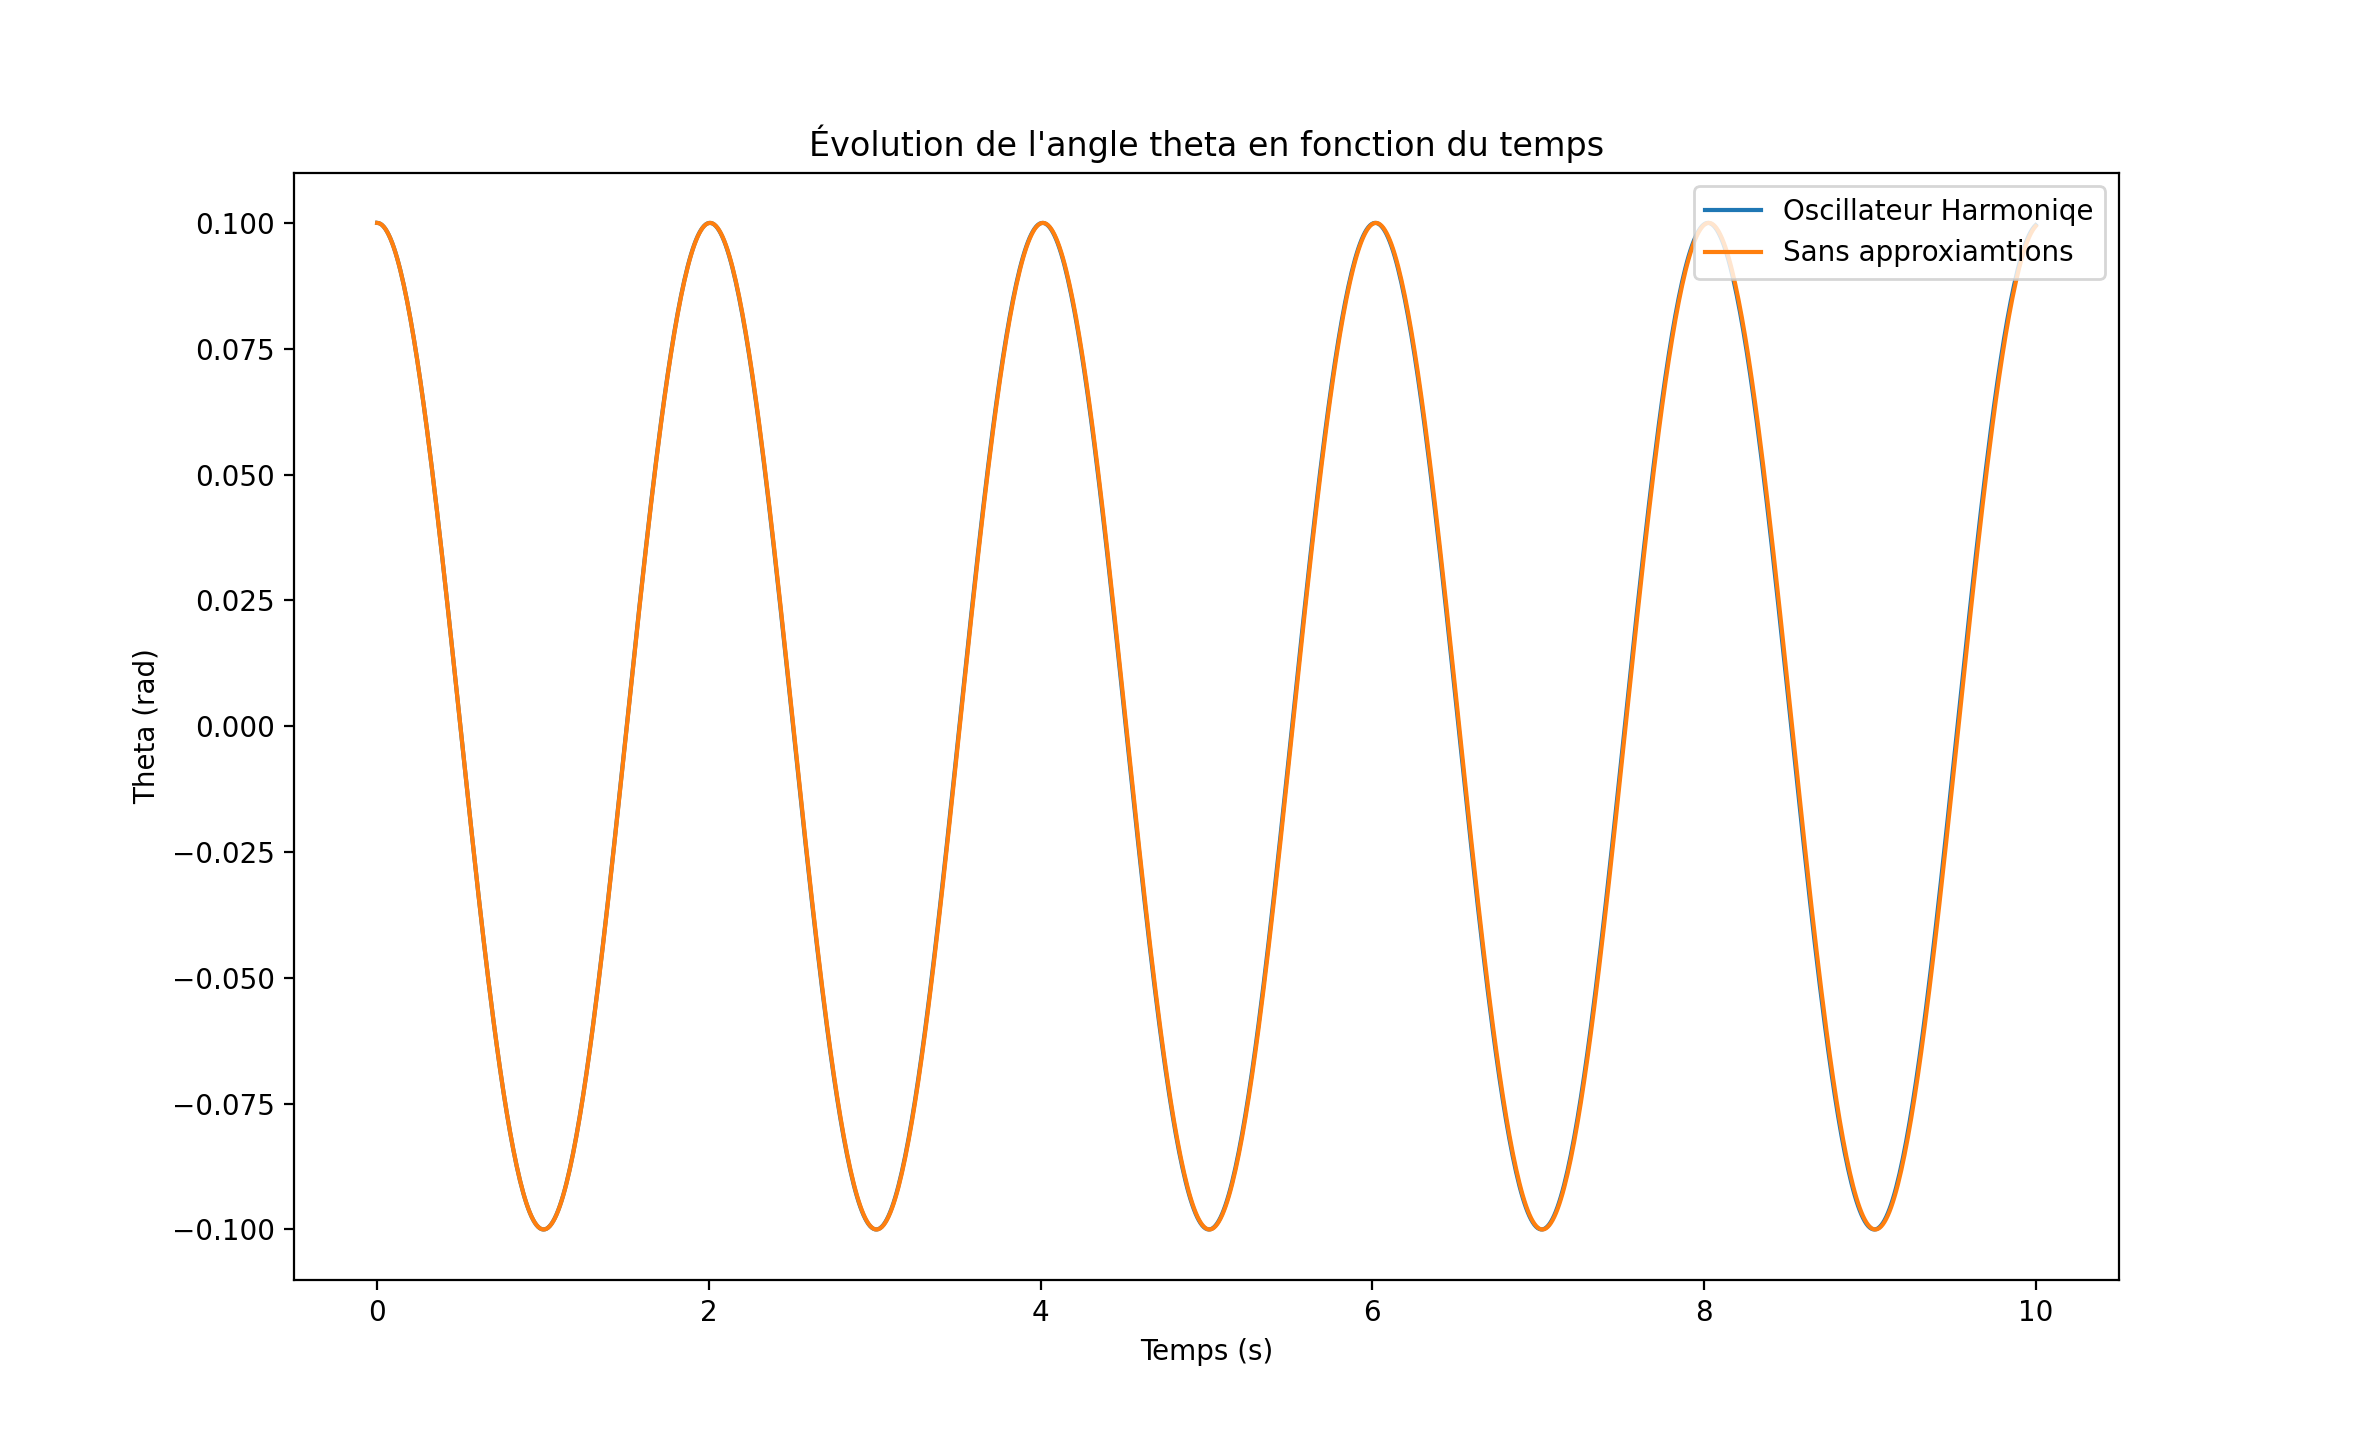
\includegraphics[scale=0.4]{./img/question7.png}\\
			\textsc{Figure 2 – } \textit{Deux simulations différentes pour les mêmes conditions initiales $\theta_0=0.1$ et $\omega_0=0$}.
		\end{center}
		\item Pour des amplitudes plus importantes, les deux simulations ne se superposent plus. Ces observations étaient attendues : en effet, pour des valeurs de $\theta_0$ très petites devant $1$, l'approximation des petits angles donnent des résultats satisfaisants; mais plus l'angle de départ est important, plus les erreurs dues à l'approximation sont importantes : la simulation n'est plus aussi réaliste qu'on ne le voudrait.
		\item On représente les résultats numériques dans une même figure : 
		\begin{center}
			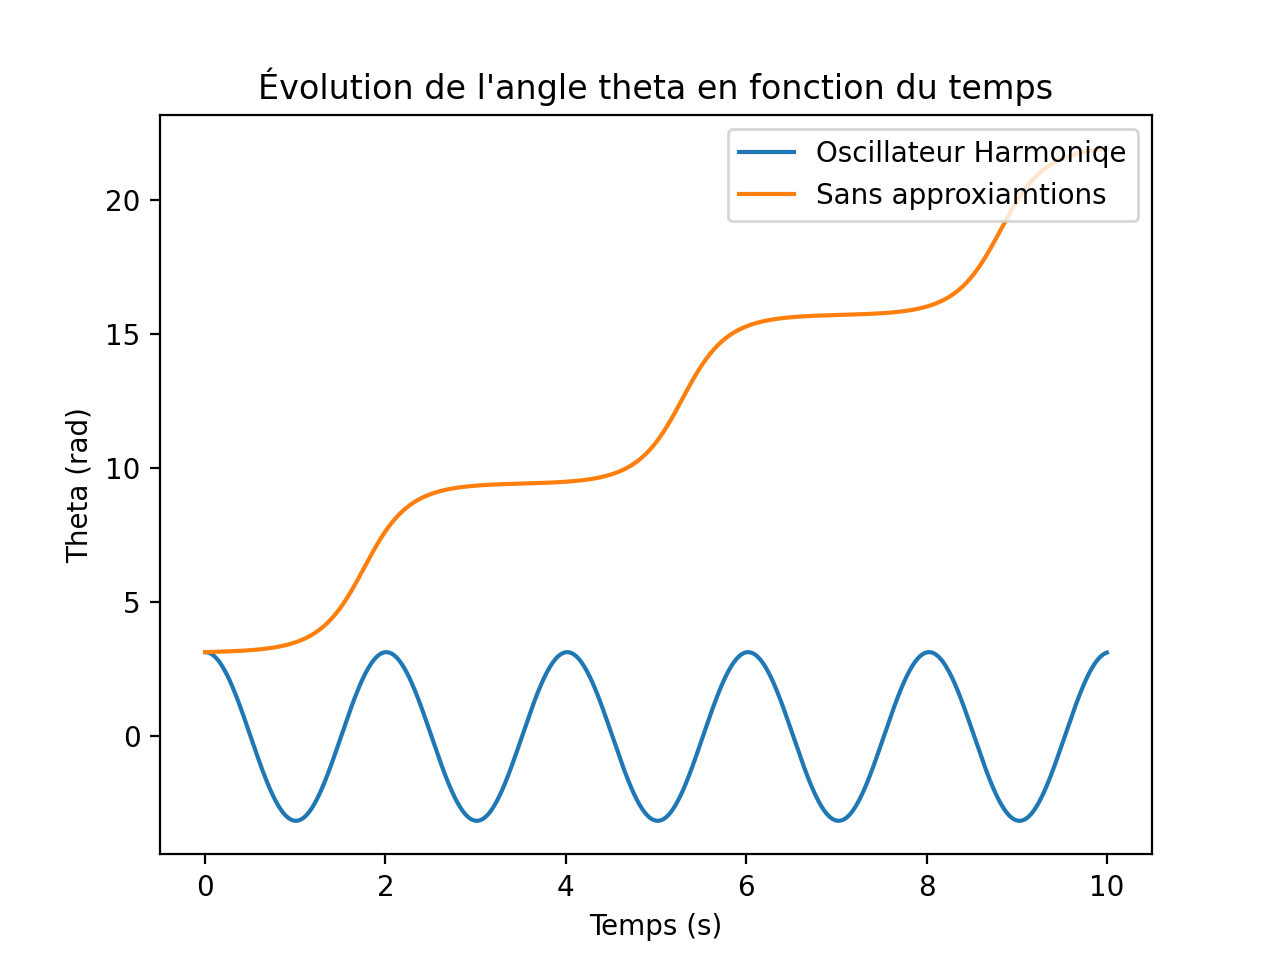
\includegraphics[scale=0.4]{./img/question9.png}\\
			\textsc{Figure 3 – } \textit{Deux simulations différentes pour les mêmes conditions initiales $\theta_0=\pi$ et $\omega_0=0.1$}.
		\end{center}
		L'évolution de l'oscillateur harmonique ne diffère pas énormément de ce que l'on a pu observer jusqu'ici avec nos simulations : la période reste la même, l'évolution temporelle de l'angle $\theta$ représente une sinusoïde. La résolution numérique de l'équation non-approximée donne des résultats drastiquement différents : non seulement la période est différente, mais l'allure de la courbe n'est plus du tout sinusoïdale; physiquement, les données traduisent une rotation indéfinie du pendule autour de l'origine, avec un ralentissement lorsque la masse est au sommet (prévisible, vue la présence du poids).
		\item On écrit la fonction suivante qui renverra la valeur de la période pour une valeur de \f{theta\_0} donnée et pour un tableau \f{t} de temps donné : 
		\begin{lstlisting}
			def periode(theta_0, t):
			    V0 = [theta_0, 0]
			    V  = odeint(pendule, V0, t)
			    v  = V[:,0]
			    first = v[0]
			    t1 = 0
			    for i, e in enumerate(v):
			        if e*first <= 0:
			            t1 = t[i] 
			            break
			    return 4*t1
		\end{lstlisting}
		On complète la section \textit{Simulations numériques} du programme avec les variables et les tableaux dont on aura besoin pour représenter l'évolution de $T$ en fonction de $\theta_0$. En lançant le programme, on obtient 
		\begin{center}
			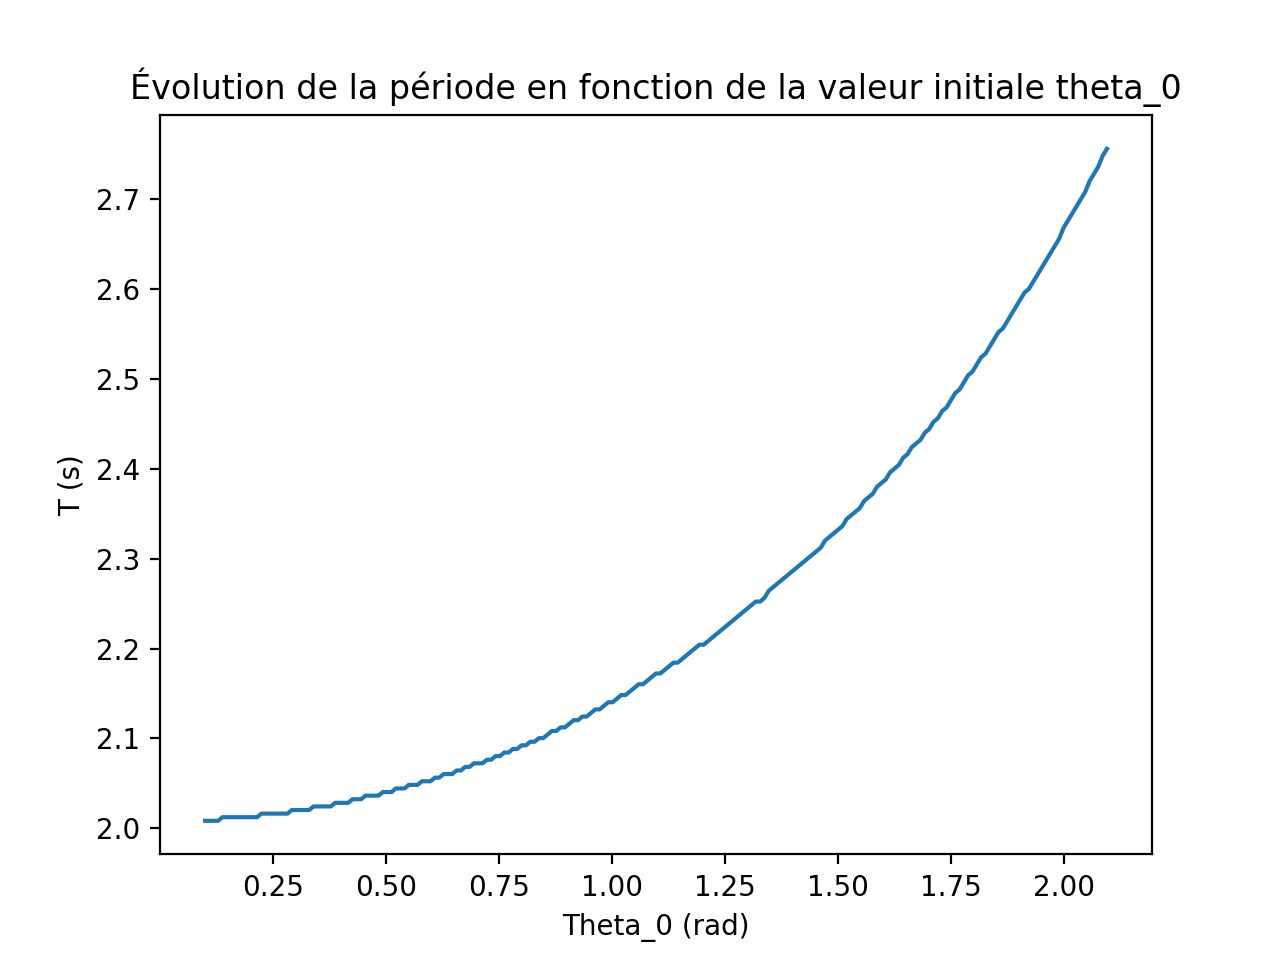
\includegraphics[scale=0.4]{./img/question10.png}\\
			\textsc{Figure 4 – } \textit{Représentation de $T(\theta_0)$}.
		\end{center}
		\item Ci-dessous, sur un même graphe, les mesures des périodes et les périodes calculées grâce à la fonction \f{borda} : 
		\begin{center}
			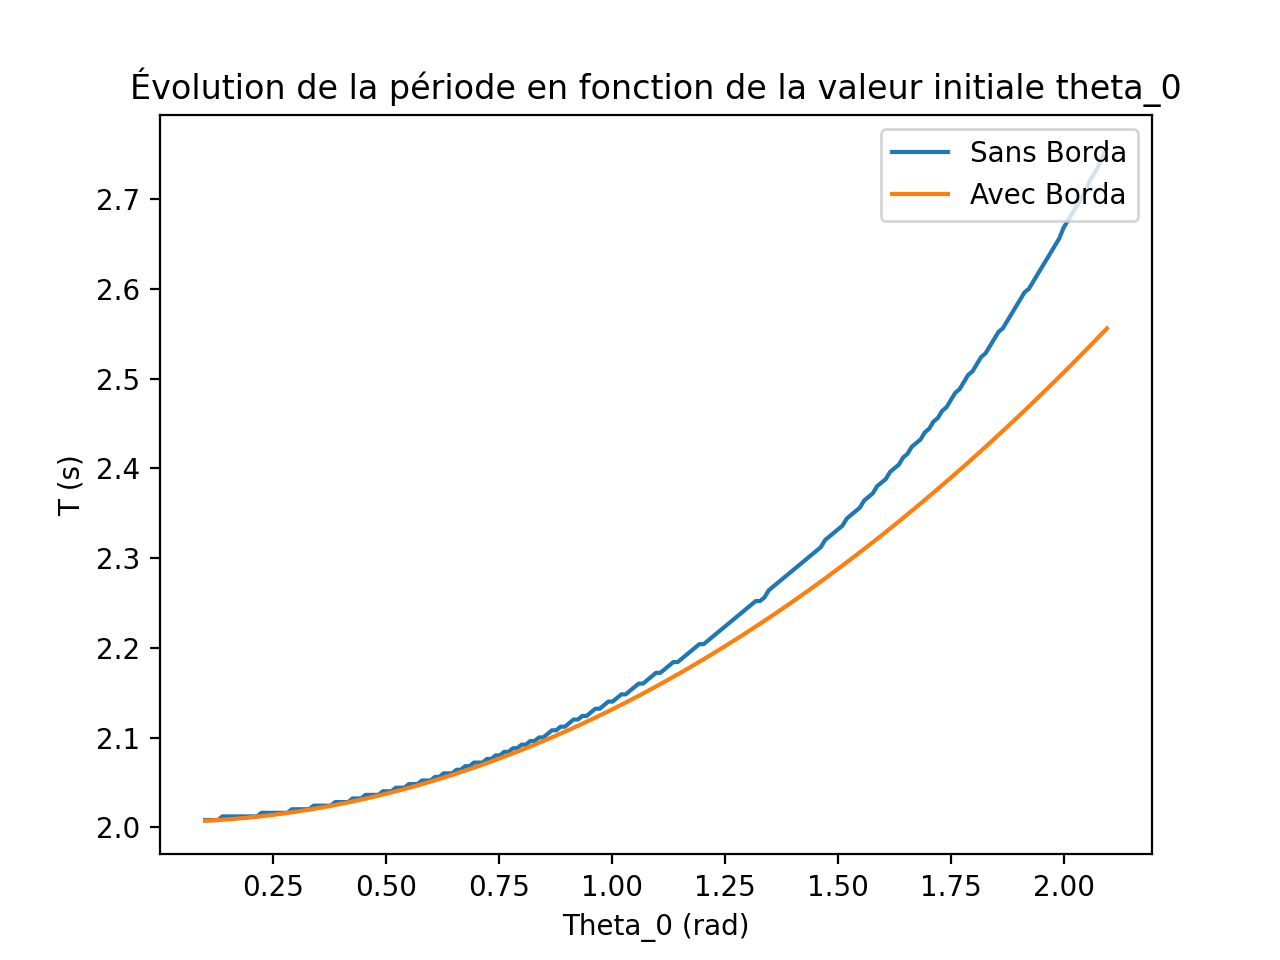
\includegraphics[scale=0.4]{./img/question11.png}\\
			\textsc{Figure 5 – } \textit{Représentations de $T(\theta_0)$}.
		\end{center}
		La fonction \f{borda} :
		\begin{lstlisting}
			def borda(theta_0):
			    return 2*np.pi*np.sqrt(l/g)(1+(theta_0**2)/16)
		\end{lstlisting}
		Pour des valeurs assez grandes de $\theta_0$, on remarque que la formule de Borda ne prédit plus très bien la valeur de $T$ pour des $\theta_0$ trop grands.
		\item On représente, en plus des deux autres \textit{versions}, le graphe de $T(\theta_0)$ obtenu à l'aide de la fonction \f{periode\_int} fournie :
		\begin{center}
			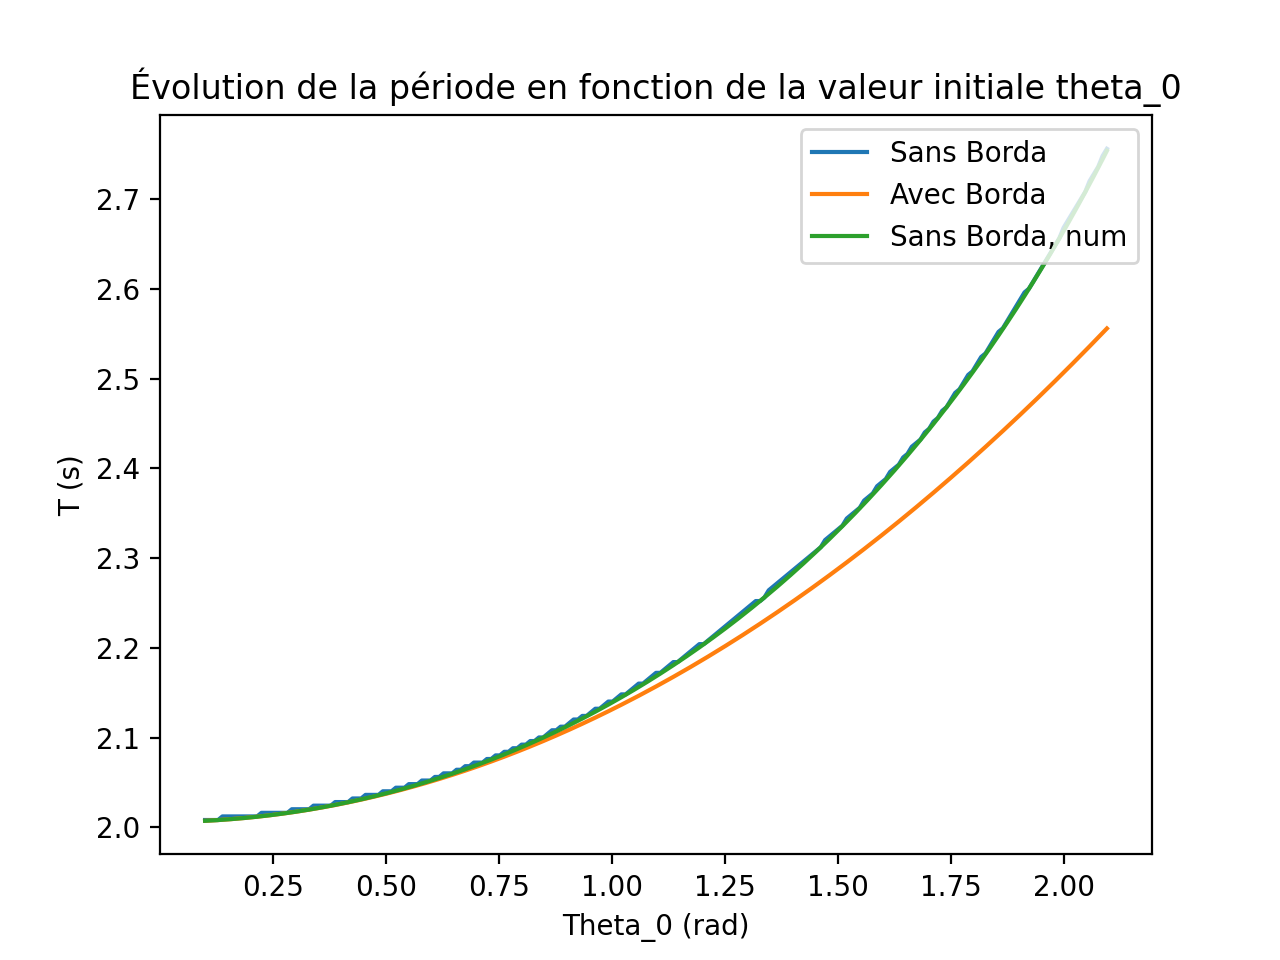
\includegraphics[scale=0.4]{./img/question12.png}\\
			\textsc{Figure 6 – } \textit{Représentations de $T(\theta_0)$}.
		\end{center}
		Le résultat obtenu se superpose quasiment avec le graphe que l'on obtient avec la fonction \f{periode}.
	\end{enumerate}

	\subsubsection*{Énergie mécanique}
	\begin{enumerate}[start=13]
		\item On a directement $\boxed{\mathcal{E}_c=\frac12ml^2\omega^2}$.
		\item On a que $\dd \mathcal{E}_p=-\delta W(\vv{P})$; on calcule : 
		\begin{align*}
			\dd \mathcal{E}_p   &= -\delta W(\vv{P})\\
								&= -\vv{P}\cdot \dd\vv{OM}\\
								&= -\vv{P}\cdot(l\dd\theta\vv{e_\theta})\\
								&= mgl\sin\theta\dd\theta
		\end{align*}
		Ainsi, on a $\mathcal{E}_p=-mgl\cos\theta+k$, $k\in\R$. On choisit $k$ tel que $\mathcal{E}_p=0$ lorsque $\theta=0$; d'où $\boxed{\mathcal{E}_p=mgl(1-\cos\theta)}$.
		\item Les fonctions sont simples et utilisent les formules obtenues analytiquement : 
		\begin{lstlisting}
			def energie_cinetique(omega):
			    return (1/2)*m*(l**2)*(omega**2)


			def energie_potentielle(theta):
			    return m*g*l*(1-np.cos(theta))


			def energie_mecanique(theta, omega):
			    return energie_cinetique(omega) + energie_potentielle(theta)
		\end{lstlisting}
		On représente l'évolution temporelle de chacune des grandeurs sur un même graphe :
		\begin{center}
			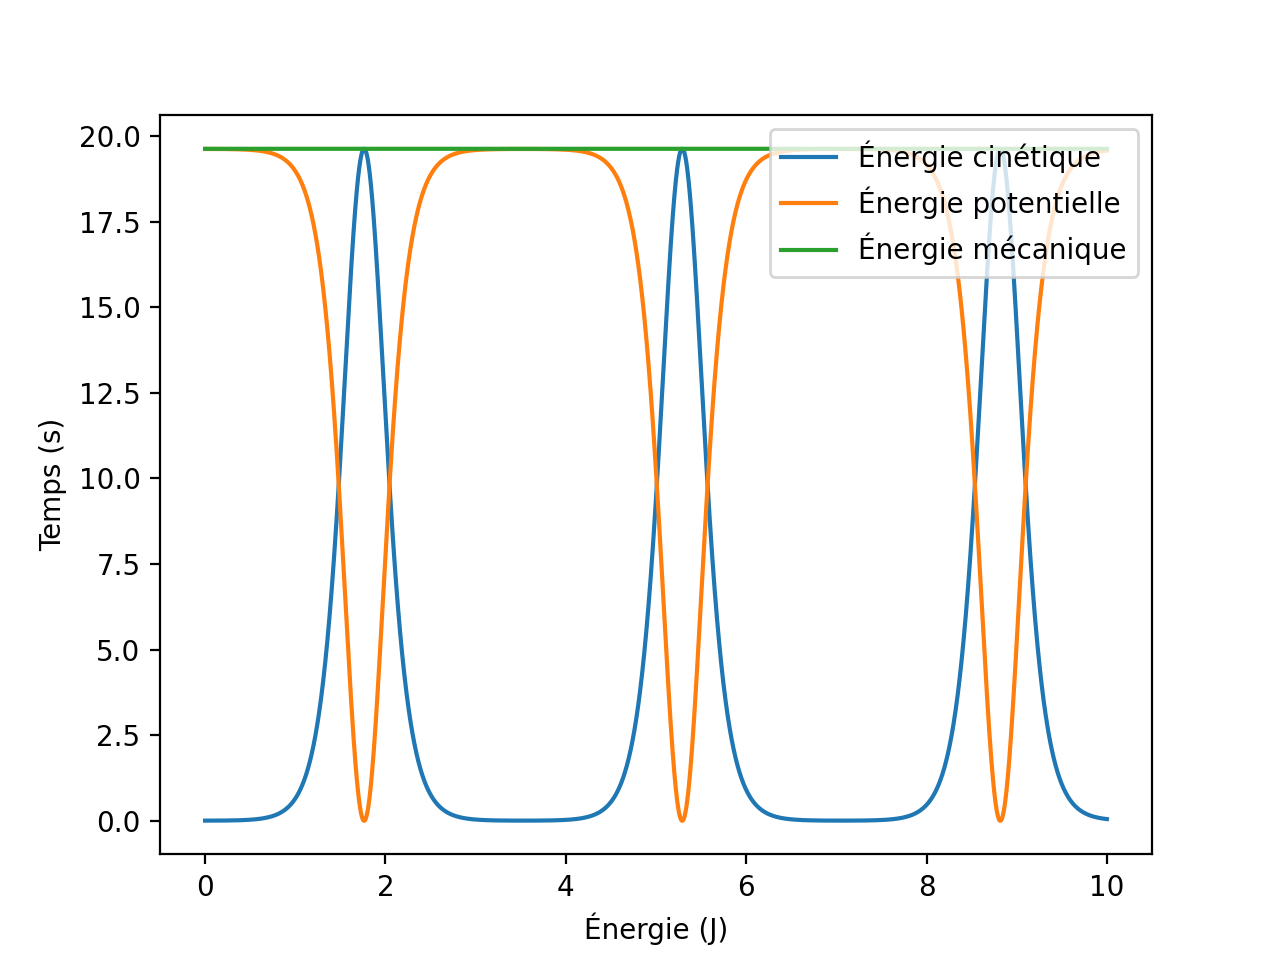
\includegraphics[scale=0.4]{./img/question15.png}\\
			\textsc{Figure 7 – } \textit{Évolutions temporelles de $\mathcal{E}_c$, $\mathcal{E}_p$ et $\mathcal{E}_m$}.
		\end{center}
		\item On résout à nouveau l'équation différentielle en s'aidant de la méthode d'Euler. On représente ensuite les énergies cinétique, potentielle et mécanique sur un même graphe. L'allule globale étant quasiment la même, on décide de zoomer sur une portion du graphe pour mettre en valeur ce qui semble être une anomalie 
		\begin{center}
			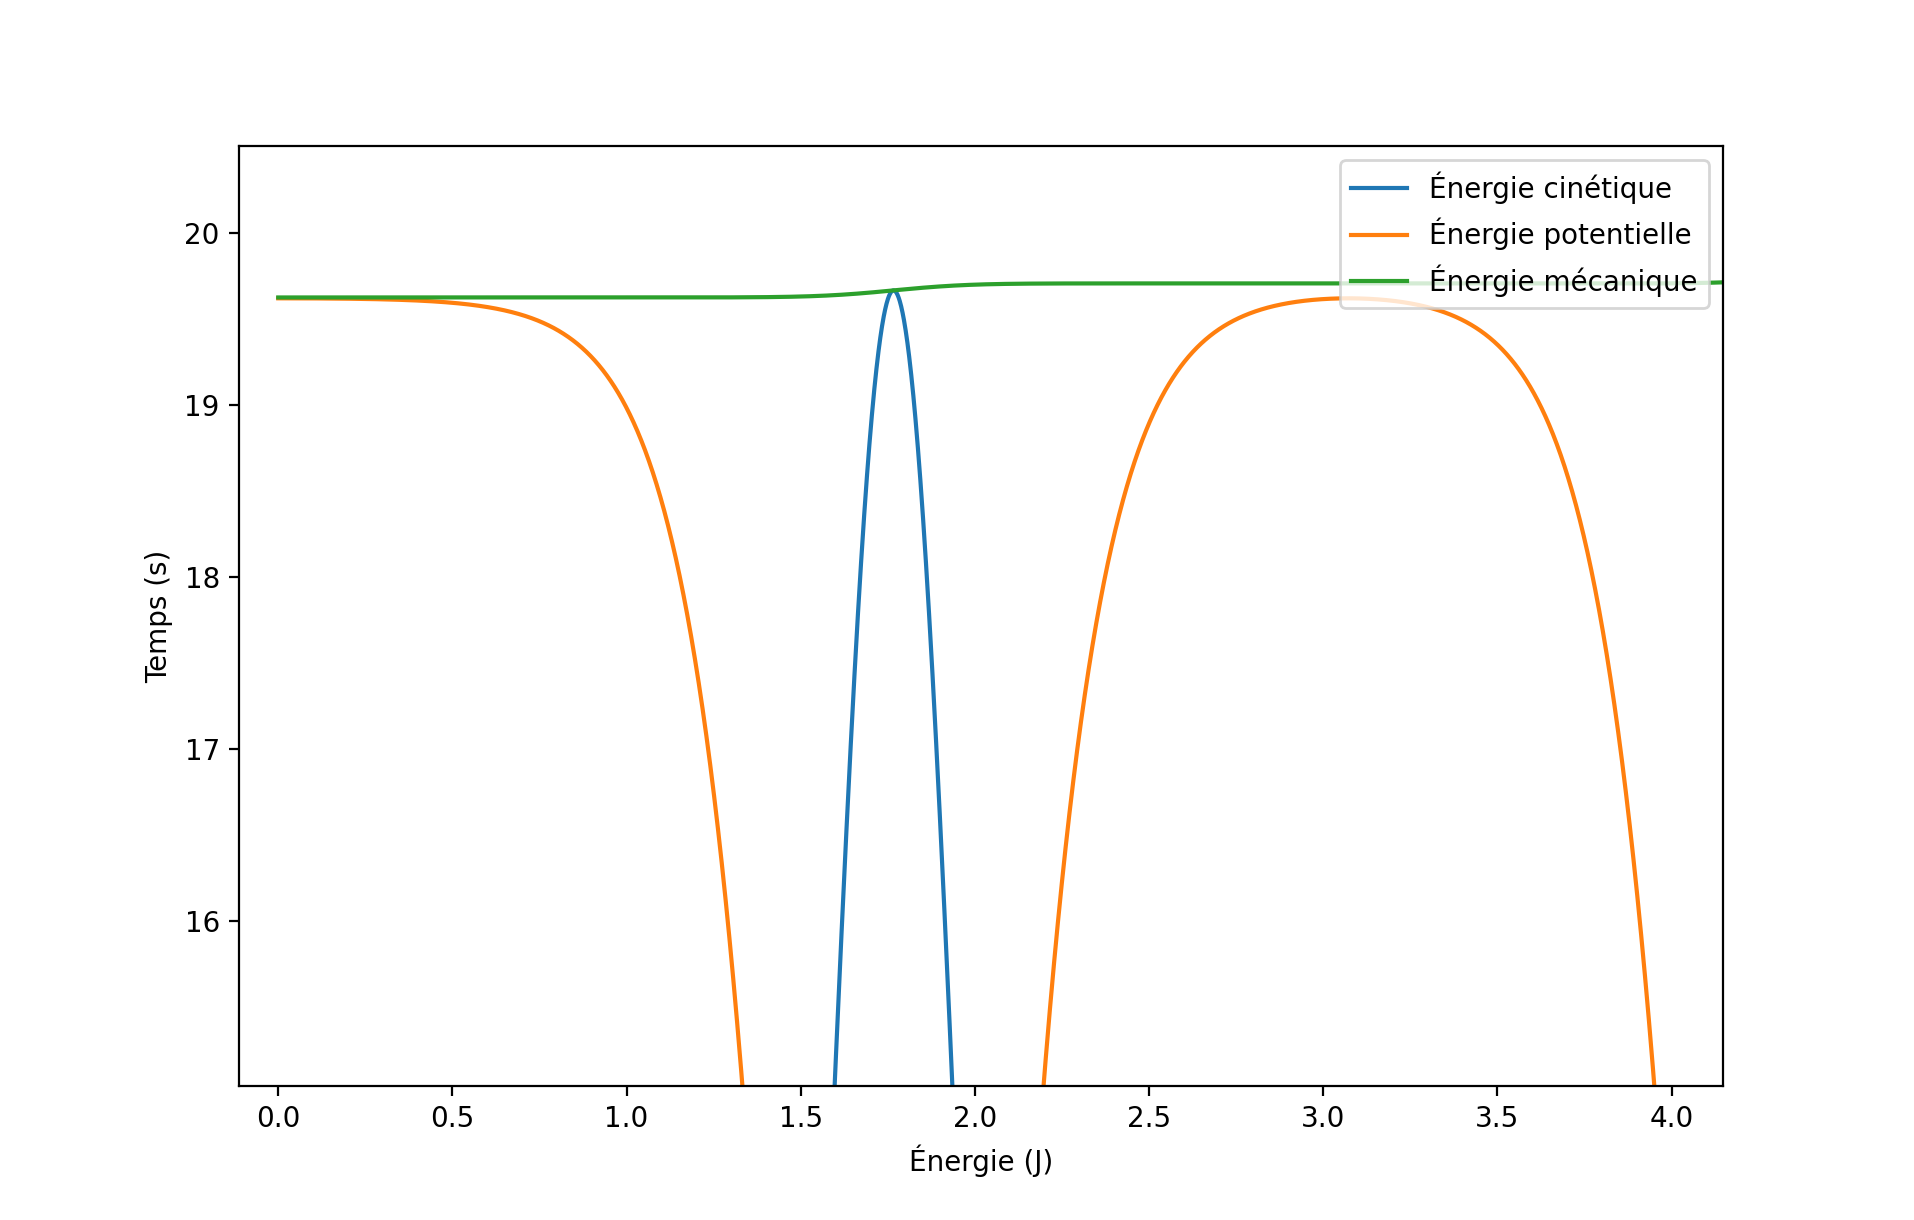
\includegraphics[scale=0.4]{./img/question16.png}\\
			\textsc{Figure 8 – } \textit{L'anomalie}.
		\end{center}
		On le remarque directement : l'énergie mécanique ne semble pas être constante; n'y a-t-il plus conservation de l'énergie mécanique ? Cela ne peut être, toutes les forces agissant sur le système sont conservatives. L'anomalie vient ici de la méthode utilisée, dont la solution donnée semble contenir trop d'erreurs.
		\item En rajoutant des frottements, on introduit un terme en $k\ell\dot{\theta}$ dans l'équation (1). On modifie la fonction \f{pendule} en conséquence : 
		\begin{lstlisting}
			def pendule(V,t):
			    """
			    Fonction associee au pendule simple
			    """
			    x, y = V
			    return [y, -(g/l)*np.sin(x)-k*l*y]
		\end{lstlisting}
		On représente enfin les énergies cinétique, potentielle et mécanique : 
		\begin{center}
			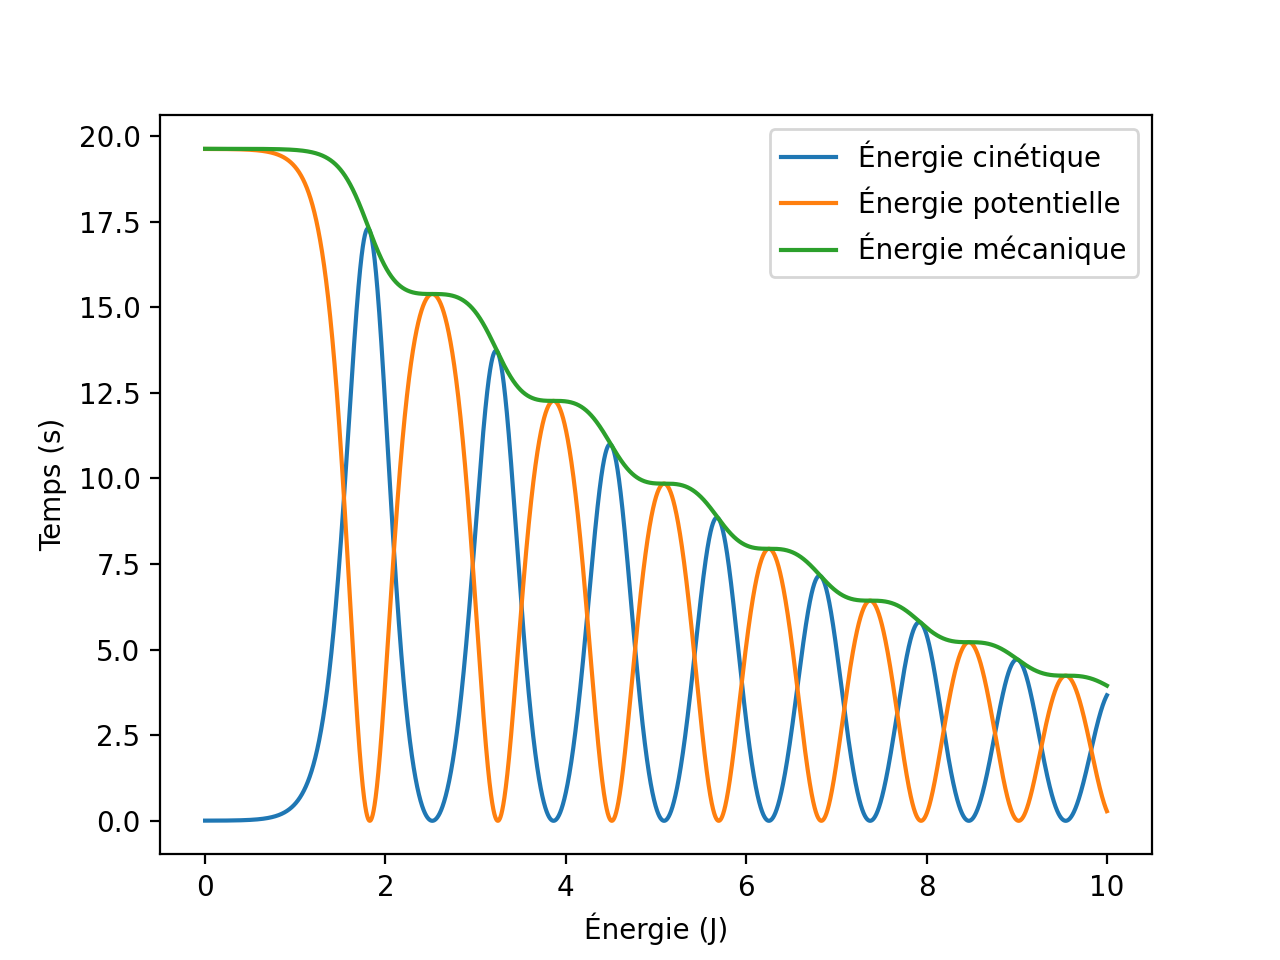
\includegraphics[scale=0.4]{./img/question17.png}\\
			\textsc{Figure 9 – } \textit{Évolutions temporelles de $\mathcal{E}_c$, $\mathcal{E}_p$ et $\mathcal{E}_m$ (avec frottements)}.
		\end{center}
		On remarque qu'il n'y a plus conservation de l'énergie mécanique : cela est du aux frottements, qui constituent une force non-conservative.
	\end{enumerate}
\end{document}

